\chapter{Исследовательская часть}

\section{Замеры времени работы}

Для замеров времени работы функции запускались 10000 раз, на каждой итерации генерировались 2 строки одинаковой длины, состоящие из случайных строчных символов английского алфавита. Результаты измерений суммировались, после чего выводилось среднее значение. Время работы было замерено с помощью функции $clock\_gettime()$ со значением первого параметра $CLOCK\_PROCESS\_CPUTIME\_ID$ \cite{clockgettime}. Все замеры проводились на ноутбуке Acer Swift 3x, процессор 11th Gen Intel(R) Core(TM) i7-1165G7 @ 2.80GHz. Во время замеров были отключены все программы, кроме Visual Studio Code.

При всех используемых вариантах замеры проводились на строках длины 2, 4, 6, 8, 10. Результаты представлены на рисунке \ref{fig:res1}.

\begin{figure}[h!]
	\centering
	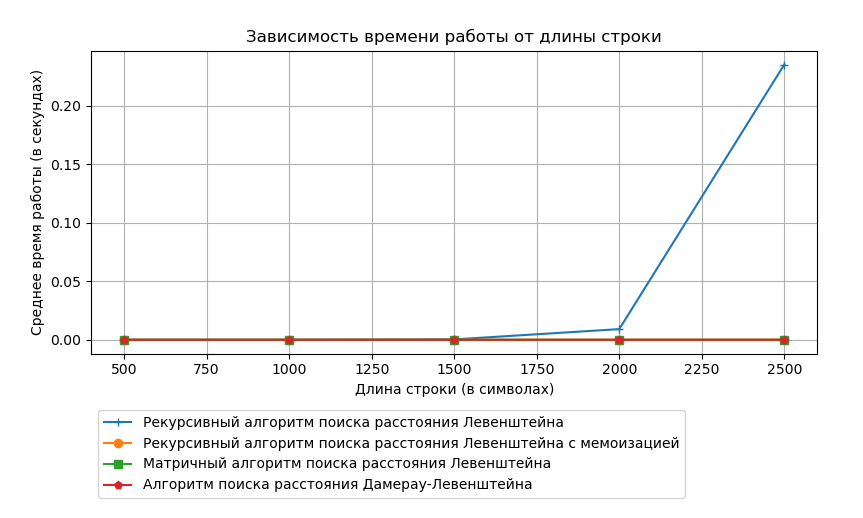
\includegraphics[width=1\textwidth]{tex_parts/research1.png}
	\caption{\label{fig:res1} Результаты замера времени работы разных алгоритмов на строках длины 2, 4, 6, 8, 10.}
\end{figure}

Как видно из результатов замера, даже при небольшом размере строки рекурсивный алгоритм поиска расстояния Левенштейна работает намного дольше остальных и не позволяет нам сравнить остальные алгоритмы между собой.

При исключении рекурсивного варианта замеры проводились на строках длины 500, 1000, 1500, 2000, 2500. Результаты представлены на рисунке \ref{fig:res2}.

\begin{figure}[h!]
	\centering
	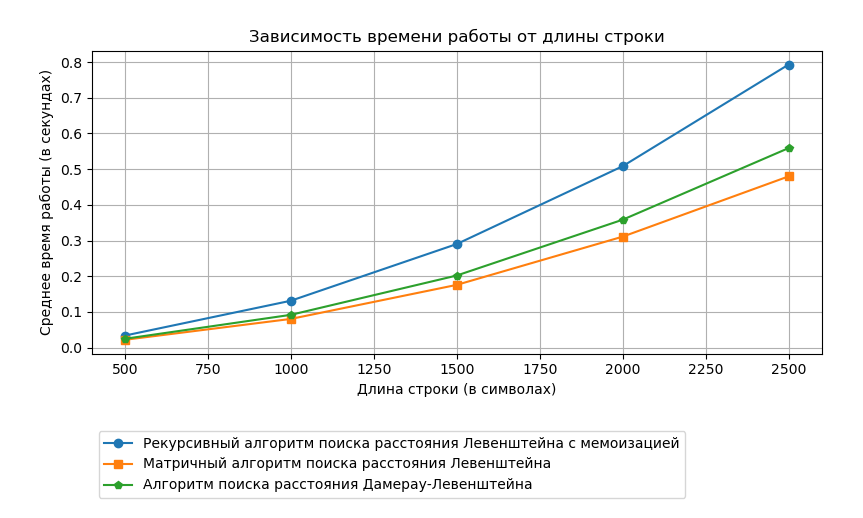
\includegraphics[width=1\textwidth]{tex_parts/research2.png}
	\caption{\label{fig:res2} Результаты замера времени работы разных алгоритмов (за исключением рекурсивного) на строках длины 500, 1000, 1500, 2000, 2500.}
\end{figure}

Наиболее эффективной по времени оказалась матричная реализация алгоритма поиска расстояния Левенштейна, после неё идёт матричная реализация алгоритма поиска расстояния Дамерау-Левенштейна, и дольше всех среди перечисленных работает рекурсивный алгоритм с мемоизацией.

\section{Вывод}

В данном разделе были проведены замеры времени. Самыми эффективными оказались матричные реализации алгоритмов, причём расстояние Левенштейна считается быстрее, чем расстояние Дамерау-Левенштейна. Далее идёт рекурсивный алгоритм с мемоизацией, и самым медленной оказалась рекурсивная реализация без мемоизации.

